\section{System Design and Architecture}
The systems' overall layered design and architecture can be seen in figures \ref{fig:LayerArchitecture} and \ref{fig:SystemArchitecture} respectively. The former provides a high-level overview of all the components in the system and the interaction between these components using various technologies. The latter, however, provides an in-depth view of the data flow and the processes in the system.

\subsection{High Level Design}
The diagram in figure \ref{fig:LayerArchitecture} shows a high-level overview of the system design. There are three main layers of the system which make up the web application. These are the:

\begin{itemize}
\item User Interface (UI) layer, developed using HTML 5 and CSS3
\item Application Services (AS) layer, responsible for performing the majority of system logic in PHP
\item Database Management System (DBMS) layer, which allows the storage and retrieval of data using MySQL
\end{itemize}

On its own, the AS layer would be insufficient to provide users with tailored content as PHP is not powerful enough to process large data quantities. For this reason, an additional `background' layer is added to the system. This layer is broken down into data collection and data analysis and will be responsible for running analysis algorithms as scheduled jobs that will analyse the data and update the database. The inclusion of this additional layer increases the efficacy of data processing, meaning the AS layer only needs to output already processed data.

\begin{figure}[H]
  \centering
  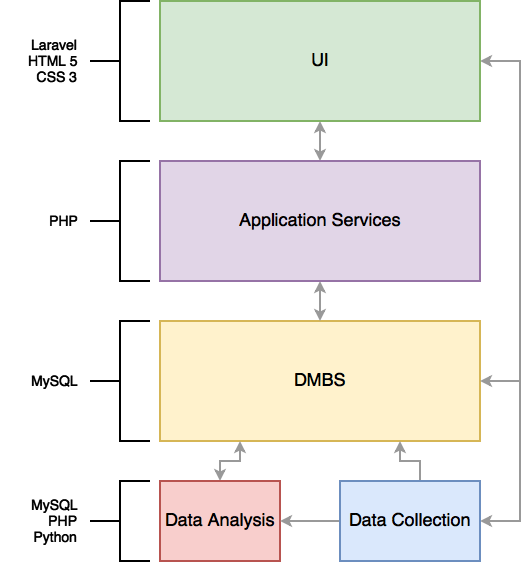
\includegraphics[width=0.5\textwidth]{Images/Design/LayerArchitecture}
  \caption{High-Level System Design} \label{fig:LayerArchitecture} 
\end{figure}

\subsection{Overall System Architecture}
The operation of the system is broken down into five stages: 

\begin{itemize}
\item Data collection
\item Data processing
\item Recommendation
\item Content filtering 
\item User interface
\end{itemize}

The functionality of each of these stages is implemented in multiple layers of the high-level system design in figure \ref{fig:LayerArchitecture}. The data collection stage will primarily be responsible for collecting data about the user, such as their personal information, as well as capturing the content, text or photos, posted by the user and storing this in the database so that it may be processed and visualised later. This raw data is represented by the black lines with arrows indicating the direction of the data flow. Additionally, the data collection process will also collect data such as tags, categories and possibly tweets from Twitter and store this so that it may be used for training machine learning models. This stage can be extended to collect data from other sources such as news feeds for better categorisation and trend plotting. The stored posts then undergo processing to assign tags explicitly used by the author, and at the same time also assign tags detected by the algorithm based on the content of the post. Once the post has been tagged, the post is assigned to a category based on its tags. The processed data, represented by green lines, is then stored in the database with state fields which indicate that the tuples have been processed. Once the data has been converted to a standard format and has been correctly associated, based on the viewers' settings, the appropriate recommendation algorithm is executed, which outputs recommended posts and users for each user. The recommended data, represented by red lines, is now held in separate data storage so that it can quickly be fetched by the server and presented to the user. However, before we can present this data to the user, we need to filter it as it may contain abusive content. This process is carried out by the content filtering stage which looks at the abuse score assigned to each post and filters out abusive posts. The abuse score is computed by a logistic regression model, in the data analysis stage in figure \ref{fig:LayerArchitecture}, trained on content from Twitter collected in the data collection stage. The original posts storage is updated at regular intervals by a scheduled job. Finally, the filtered content, represented by blue lines, can be displayed to the user on various pages and widgets throughout the site. 

\begin{figure}[H]
  \centering
  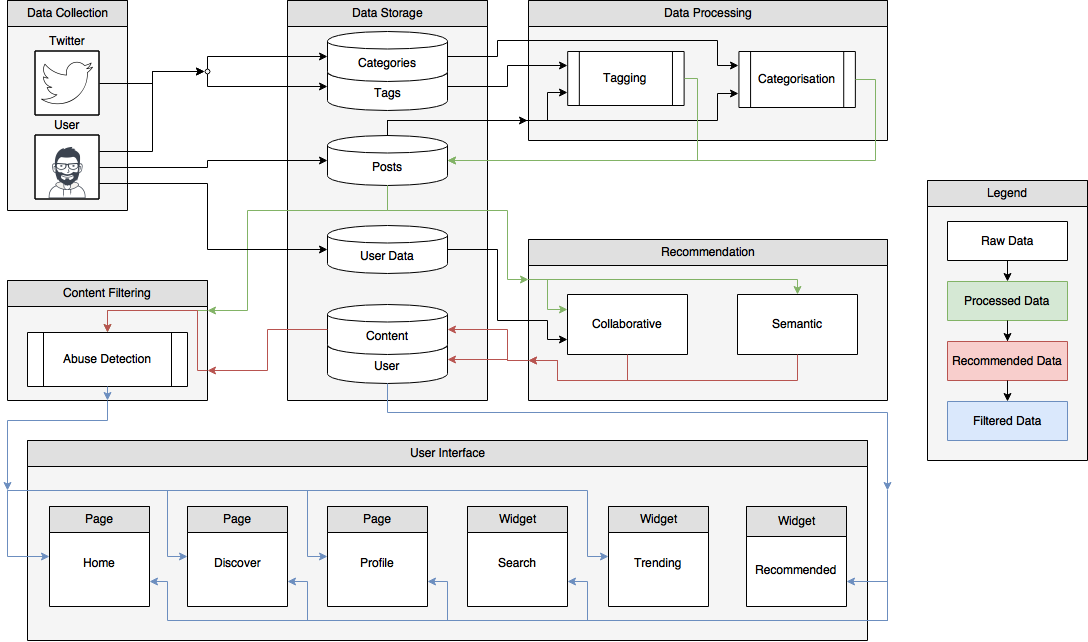
\includegraphics[width=1.0\textwidth]{Images/Design/SystemArchitecture}
  \caption{Proposed System Architecture Diagram} \label{fig:SystemArchitecture} 
\end{figure}